\chapter{Model inference for web applications}
\label{sec:modelinf:webapps}

Our target has always been to construct models of (legacy)
production systems in an automated fashion. But, before tackling
the model inference of production systems, we chose to validate
our initial ideas and concepts by applying them on web
applications. Given a black-box approach, web applications are
often smaller and less complex than production systems: no
physical devices involved, a well-known client-server
architecture, and a well-defined protocol to exchange
information. The purpose of this chapter is to present the
premises of our work on model inference (of production systems)
applied to web applications.

In this chapter, we introduce the first version of
\textit{Autofunk}, our modular framework for inferring models,
\emph{i.e.} Input/Output Symbolic Transition Systems here, by
using a rule-based expert system. A bisimulation minimization
technique \cite{Park:1981:CAI:647210.720030} is applied to reduce
the model size. We generate several models of a same application
at different levels of abstraction. \textit{Autofunk} relies on
an \emph{automatic testing} technique to improve the completeness
of the inferred models. We evaluate our tool on the
GitHub\footnote{\url{https://github.com/}} website, showing
encouraging results.\\

\minitoc

\pagebreak

\section{Introduction}

Web applications are often smaller and easier to understand than
production systems. The design of web applications is
well-established: we have a web server that runs the application,
no matter its underlying programming language, and a client (a
web browser most of the time) that connects to the web server so
that it can talk to the application. \textit{Hypertext Transfer
Protocol} (HTTP)  is the protocol that allows such a discussion by
means of HTTP requests and HTTP responses \cite{RFC7230}.
Usually, the client initiates a request, and the server responds
to it. That is why we consider web applications as event-driven
applications: they react to events. Requests embed HTTP verbs (or
methods), \textit{Unique Resource Identifiers} (URIs also known
as the "web links"), and sometimes parameters along with their
values. When one submits a registration form on a web page, it is
likely that the HTTP verb is $POST$, and that there are at least
as many parameters and values as fields in the form. By clicking
on the "submit" button (or "save", "register", etc.), the web
browser crafts an HTTP request containing all the information,
and sends it to the web server that delivers the request to the
application. When the application sends back the appropriate
response, it also goes through the web server. By hooking between
the web browser and the web server, we are able to read both HTTP
requests and responses as far as there is no \textit{Secure
Socket Layer} (SSL) or \textit{Transport Layer Security} (TLS)
involved, \emph{i.e.} the communication channel should not be encrypted.

The information collected by reading HTTP requests and HTTP
responses are known as (HTTP) \textit{traces}. We use such traces
(and the underlying knowledge) to infer raw models of the
behaviors of a web application. We then construct more abstract
models that can be used for different purposes, \emph{e.g.},
documentation or test case generation. We chose to work on this
to explore different options for production systems in the
future. We present an active technique that uses automatic
testing to stimulate the web application in order to enhance the
completeness of the inferred models.

We start by giving an overview of this framework called
\emph{Autofunk} in the next section, which we describe in Section
\ref{sec:modelinf:webapps:contrib}.  We present our results in
Section \ref{sec:modelinf:webapps:exp}, and we conclude on this
chapter in Section \ref{sec:modelinf:webapps:conclusion}.

\textbf{Publications.} This work has been published in
\emph{Actes de la 13eme {\'e}dition d’AFADL, atelier francophone
sur les Approches Formelles dans l’Assistance au
D{\'e}veloppement de Logiciels} (AFADL'14)
\cite{durand2014inference}, and in the Proceedings of the Fifth
Symposium on Information and Communication Technology (SoICT'14)
\cite{DBLP:conf/soict/DurandS14}.

%%%%%%%%%%%%%%%%%%%%%%%%%%%%%%%%%%%%%%%%%%%%%%%%%%%%%%%%%%%%%%%%%

\section{Overview}

We propose a new approach to infer models of web applications,
which is divided into several modules as depicted in Figure
\ref{fig:soict-framework}. The \textit{Models generator} is the
centerpiece of this framework. It takes HTTP traces as inputs,
which can be sent by a \textit{Monitor} collecting them on-the-fly.
Such a monitor would be responsible for reading HTTP requests and
responses in our case. Nonetheless, it is worth mentioning that the
traces can also be sent by any tool or even any user, as far as
they comply to a chosen standard format like \textit{HTTP
Archive} (HAR), which is implemented in recent browsers'
developer tools. The Models generator is based upon an expert
system, which is an artificial intelligence engine emulating acts
of a human expert by inferring a set of rules representing his
knowledge.  Such knowledge is organized into a hierarchy of
several layers.  Each layer gathers a set of inference rules
written with a first-order logic. Typically, each layer creates a
model, and the higher the layer is, the more abstract the model
becomes. Models are then stored and can be later analyzed by
experts, verification tools, etc. The number of layers is not
strictly bounded even though it is manifest that it has to be
finite.

\begin{figure}[ht]
    \begin{center}
        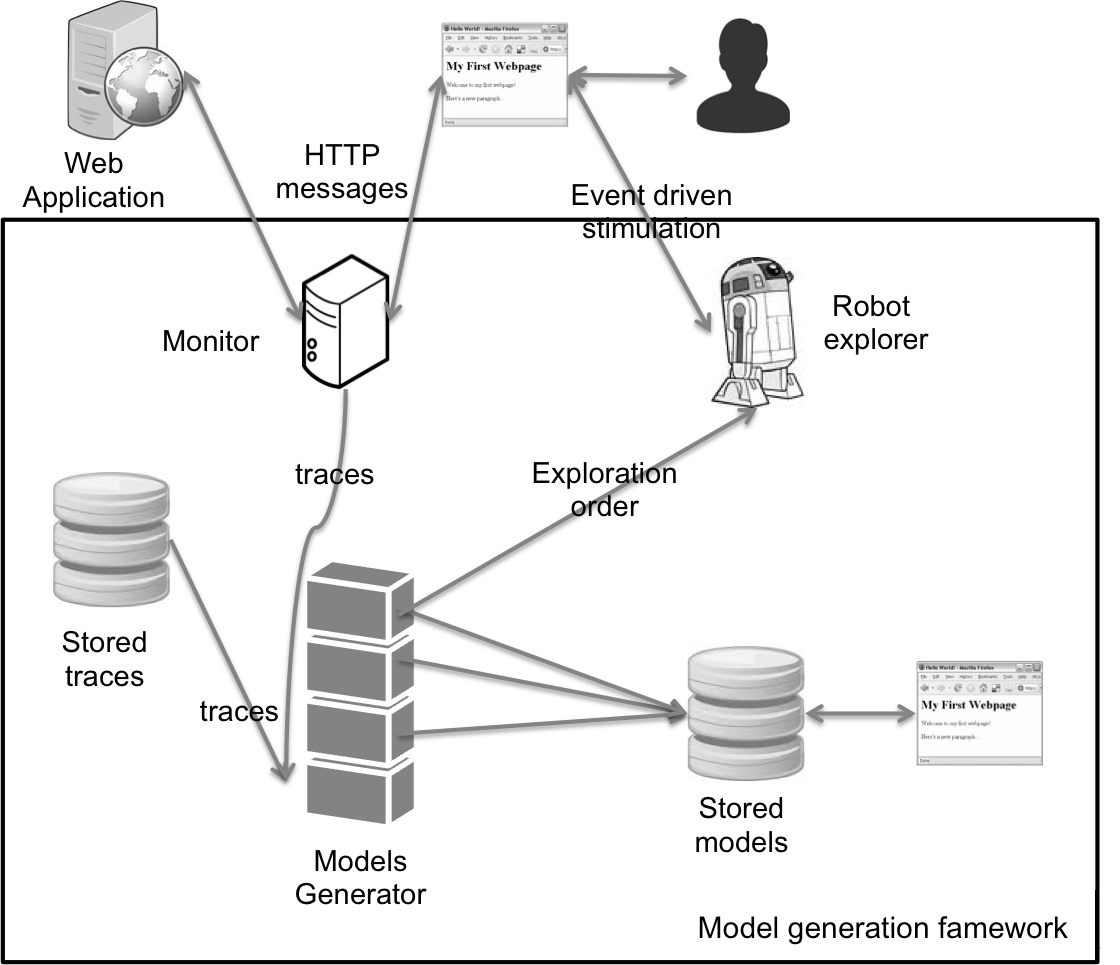
\includegraphics[width=0.8\linewidth]{figures/soict-framework.png}
    \end{center}

    \caption{Very first overall architecture of \textit{Autofunk}, our
    model generation framework for web applications.}
    \label{fig:soict-framework}
    \TODO{to redraw}
\end{figure}

The Models generator relies upon traces to construct IOSTSs (cf.
\crossref{sec:related}{sec:definitions:iosts}), but the given
trace set may not be substantial enough to generate relevant
IOSTSs. More traces could be yet collected as far as the
application being analyzed is an event-driven application.  Such
traces can be produced by stimulating and exploring the
application with automatic testing. In our approach, this
exploration is achieved by the \textit{Robot explorer}, which is
our second main contribution in this framework. In contrast with
most of the existing crawling techniques, which are detailed in
\crossref{sec:related}{sec:active-crawling}, our robot does not
cover the application in blind mode or with a static traversal
strategy.  Instead, it is cleverly guided by the Models
generator, which applies an exploration strategy carried out by
inference rules.  This involves the capture of new traces by the
Monitor or by the Robot explorer that returns them to the Models
generator. The advantages of this approach are manifold:

\begin{itemize}
\item It takes a predefined set of traces collected from any kind
of applications producing traces. In the context of web
applications, traces can be produced using automatic testing;

\item The application exploration is guided with a strategy that
can be modified according to the type of application being
analyzed. This strategy offers the advantage of directly targeting
some states of the application when its state number is too large
for being traversed in a reasonable processing time. Strategies
are defined by means of inference rules;

\item The knowledge encapsulated in the expert system can be used
to cover trace sets of several applications thanks to generic
rules. For instance, the same rules can be applied to the
applications developed with the same framework or programming
language;

\item But, the rules can also be specialized and refined for one
application to yield more precise models. This is interesting for
application comprehension;

\item Our approach is both flexible and scalable. It does not
produce one model but several ones, depending on the number of
layers of the Models generator, which is not limited and may
evolve in accordance to the application's type. Each model,
expressing the application's behaviors at a different level of
abstraction, can be used to ease the writing of complete formal
models, to apply verification techniques, to check the
satisfiability of properties, to automatically generate
functional test cases, etc.
\end{itemize}

In the following section, we describe our model inference method.

%%%%%%%%%%%%%%%%%%%%%%%%%%%%%%%%%%%%%%%%%%%%%%%%%%%%%%%%%%%%%%%%%

\section{Inferring models with rule-based expert systems}
\label{sec:modelinf:webapps:contrib}

The Models generator is mainly composed of a rule-based expert
system, adopting a forward chaining. Such a system separates the
knowledge base from the reasoning: the former is expressed with
data also known as facts and the latter is realized with
inference rules that are applied to the facts. Our Models
generator initially takes traces as an initial knowledge base and
owns inference rules organized into layers for trying to fit the
human expert behavior. These layers are depicted in Figure
\ref{fig:se}.

\begin{figure}[ht]
    \begin{center}
        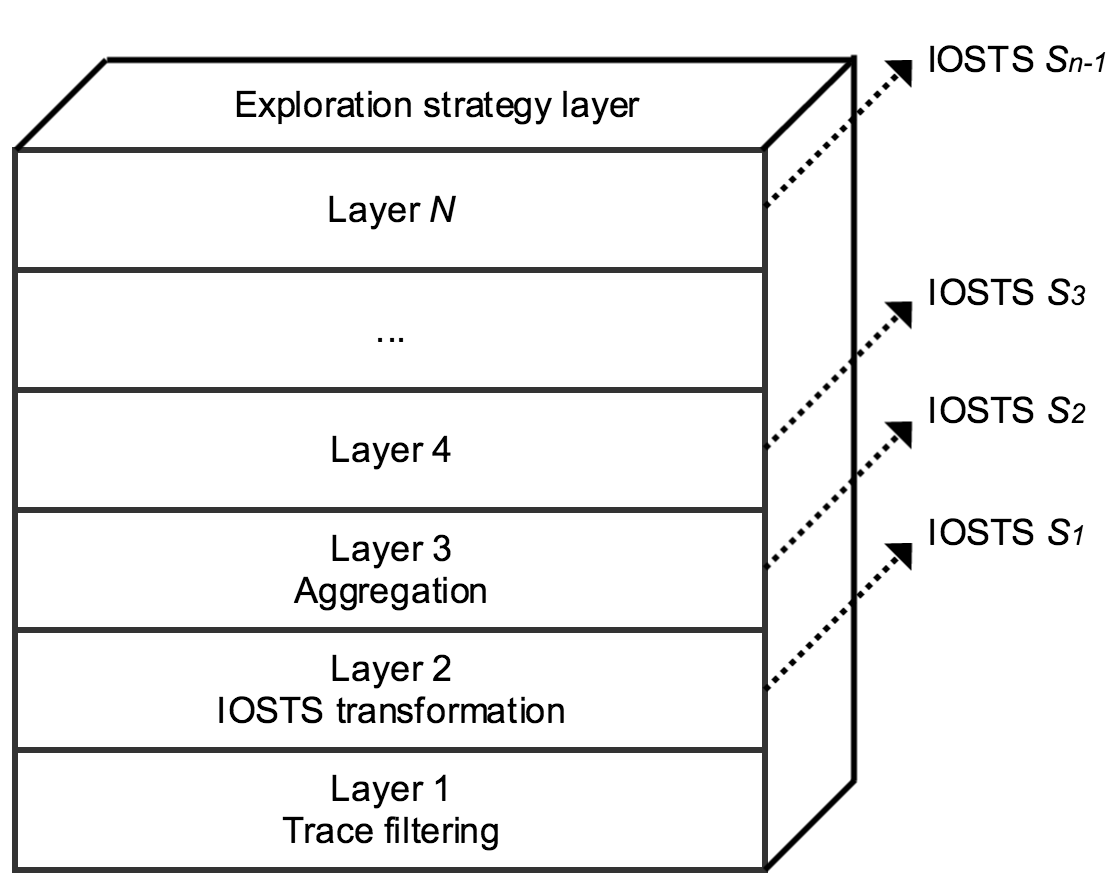
\includegraphics[width=1.0\linewidth]{figures/soict_se.png}
    \end{center}

    \caption {The Models generator stack. Each layer yields a
    model that is reused by the next layer to yield another
    model, and so on. An orthogonal layer describes any kind of
    exploration strategy by means of rules.}
    \label{fig:se}
\end{figure}

Usually, when a human expert has to read traces of an
application, he often filters them out to only keep those that
make sense against the current application. This step is done by
the first layer whose role is to format the received HTTP traces
into sequences of valued actions and to delete those considered
as unnecessary. The rules of this layer depend on the nature of
the input traces. The resulting structured trace set, denoted by
$ST$, is then given to the next layer. This process is
incrementally done, \emph{i.e.} every time new traces are given to the
Models generator, these are formatted and filtered before being
given to Layer 2. The remaining layers yield an IOSTS each
$\EuScript{S}_i (i\geq 1)$, which has a tree structure derived
from the traces. The role of Layer 2 is to carry out a first
IOSTS transformation from the structured traces of $ST$, and then
to yield a minimized IOSTS $\EuScript{S}_1$. The next layers
3 to N (with N a finite integer) are composed of rules that
emulate the ability of a human expert to simplify transitions, to
analyze the transition syntax for deducing its meaning in
connection with the application, and to construct more abstract
actions that aggregate a set of initial ones. Theses deductions
are often not done in one step. This is why the Models generator
supports a finite but not defined number of layers.  Each of
these layers $i$ takes the IOSTS $\EuScript{S}_{i-1}$ given by
the direct lower layer. This IOSTS, which represents the current
base of facts, is analyzed by the rules of a expert system to
infer another IOSTS whose expressiveness is more abstract than
the previous one. We state that the lowest layers (at least Layer
3) should be composed of generic rules that can be reused on
several applications of the same type. In contrast, the highest
layers should own the most precise rules that may be dedicated to
one specific application.

For readability purpose, we chose to represent inference rules
with the
\emph{Drools}\footnote{\url{http://www.jboss.org/drools/}} rule
inference language. A \emph{Drools rule} has the following rough
structure:

\begin{BVerbatim}
rule "name"
  when
    LHS
  then
    RHS
end
\end{BVerbatim}

$LHS$ stands for Left-Hand Side. It is the conditional part of
the rule, containing the \emph{premises} of the rule. $RHS$ is
the Right-Hand Side of the rule, \emph{i.e.} the actions that are
executed (also known as conclusions) whenever $LHS$ is evaluated
to true. The rule above could have been expressed as follows:
$\frac{LHS}{RHS}$, but for more complex rules, the Drools
formalism is more readable. Furthermore, one of the biggest
advantages of Drools is its ability to handle structured data as
facts, such as Java objects.

Independently on the application's type, Layers 2 to N handle the
following fact types: \textit{Location}, which represents an
IOSTS location, and \textit{Transition}, which represents an
IOSTS transition composed of two locations $Linit$, $Lfinal$,
and two data collections \textit{Guard} and \textit{Assign}. It
is manifest that the inference of models has to be done in a
finite time and in a deterministic way, otherwise our solution
may not be usable in practice. To reach that purpose, we
formulate the following hypotheses on the inference rules:

\begin{enumerate}
    \item \textbf{Finite complexity:} a rule can only be applied
        a limited number of times to the same knowledge base;

    \item \textbf{Soundness:} the inference rules are Modus
        Ponens, \emph{i.e.} simple implications that lead to
        sound facts if the original facts are true (P implies Q;
        P is asserted to be true, so therefore Q must be true.);

    \item \textbf{No implicit knowledge elimination:} after the
        application of a rule $r$ expressed by the relation $r:
        T_i \rightarrow T_{i+1} (i\geq 2)$, with $T_i$ a
        transition base, for $t=(l_n,l_m,a(p),G,A)$ extracted
        from $T_{i+1}$, $l_n$ is reachable from $l0$.
\end{enumerate}

In the following, we illustrate each layer with examples.

\subsection{Layer 1: Trace filtering}
\label{sec:modelinf:webapps:L1}

Traces of web applications are based upon the HTTP protocol,
conceived in such a way that each HTTP request is followed by
only one HTTP response. Consequently, the traces, given to Layer
1, are sequences of couples (HTTP request, HTTP response). This
layer begins formatting these couples so that these can be
analyzed in a more convenient way.

An HTTP request is a textual message containing an HTTP verb
(also called method), followed by a Unique Resource Identifier
(URI). It may also contain header sections such as Host,
Connection, or Accept. The corresponding HTTP response is also a
textual message containing at least a status code. It may
encompass headers (\emph{e.g.},  Content-Type, Content-Length) and a
content. All these notions can be easily identified. For
instance, Figure \ref{fig:httpexample} depicts an HTTP request
followed by its response. This is a $GET$ HTTP request, meaning a
client wants to read the content of the $/hello$ resource, which
is, in this case, a web page in HTML.

\begin{figure}[ht]
\begin{framed}
\begin{BVerbatim}
GET /hello HTTP/1.1
Host: example.org
Connection: keep-alive
Accept: text/html
\end{BVerbatim}
\end{framed}

\begin{framed}
\begin{BVerbatim}
HTTP/1.1 200 OK
Content-Type: text/html
Content-Length: 13
Hello, World!
\end{BVerbatim}
\end{framed}

    \caption{An example of HTTP request and response. HTTP messages
    are sent in plain text, according to RFC 7230 \cite{RFC7230}.}
    \label{fig:httpexample}
\end{figure}

For a couple \textit{(HTTP request, HTTP response)}, we extract
the following information: the HTTP verb, the target URI, the
request content that is a collection of data (headers, content),
and the response content that is the collection (HTTP status,
headers, response content). A header may also be a collection of
data or may be null. Contents are textual, \emph{e.g.}, HTML.
Since we wish to translate such traces into IOSTSs, we turn these
textual items into a structured \emph{valued action}
$(a(p),\theta)$ with $a$ the HTTP verb and $\theta$ a valuation
over the variable set $p=\{URI,request,response\}$. This is
captured by the following definition:

\begin{definition}[Structured HTTP traces] Let $t=
req_1,resp_1$, \dots, $req_n,$ $resp_n$ be a raw HTTP trace
composed of an alternate finite sequence of HTTP request $req_i$
and HTTP response $resp_i$. The structured HTTP trace $\sigma$ of
$t$ is the sequence of valued actions $\sigma(t) =
(a_1(p),\theta_1) \dots (a_n(p),\theta_n)$ where:

\begin{itemize}
    \item $a_i$ is a HTTP verb used to make the request in
        $req_i$;

    \item $p$ is a parameter set $\{URI, request, response\}$;

    \item $\theta_i$ is a valuation $p \rightarrow D_p$ that
        assigns a value to each variables of $p$.  $\theta$ is
        deduced from the values extracted from $req_i$ and
        $resp_i$.
\end{itemize}

The resulting structured HTTP trace set derived from the raw HTTP
traces is denoted by $ST$.
\end{definition}

If we take back the HTTP messages given in Figure
\ref{fig:httpexample}, we obtain the structured HTTP trace
$\sigma = (Get(p), \theta)$ with $\theta = \{URI="/hello",
request=\{headers=[ Host = "example.org", Connection =
"keep-alive", Accept = "text/html" ]\},\\
response = \{status\_code = 200, headers=[ Content-Type =
"text/html",\\
Content-Length = 13], content = "Hello, World!"\}\}$.

For a main request performed by a user, many other sub-requests
are also launched by a browser in order to fetch images,
CSS\footnote{Cascading Style Sheets} and JavaScript files.
Generally speaking, these do not enlighten a peculiar functional
behavior of the application. This is why we propose to add rules
in Layer 1 to filter these sub-requests out from the traces. Such
sub-requests can be identified by different ways, \emph{e.g.}, by
focusing on the file extension found at the end of the URI or on
the content-type value of the request headers.  Consequently,
this layer includes a set of rules, constituted of conditions on
the HTTP content found in an action, that remove valued actions
when the condition is met.

A straightforward rule example that removes the actions relative
to the retrieval of PNG\footnote{Portable Network Graphics}
images, and written with the Drools formalism, is given in Figure
\ref{fig:layer1:filter}.  $\$valued\_action$ is a variable
representing a $Get$ (valued) action.  Actions own $request$ and
$response$ attributes, respectively representing the HTTP request
and HTTP response for that given valued action. Such attributes
can be accessed into the action's parentheses:
$Action(request.attr)$, where $attr$ is a request's attribute
(such as $mime\_type$ and $file\_extension$), along with logical
symbols such as $or$, $and$, and $not$. Actions can be
manipulated in the $then$ part of the rule, as shown in Figure
\ref{fig:layer1:filter}. The $retract$ keyword is used to remove
a fact from the knowledge base. This rule, which is an example of
filtering rules, could be expressed as follows:

\begin{center}
$\frac{
    \begin{matrix}
        valued\_event = (Get(p), \theta) \in \sigma,\\\theta
        \models [ (request.mime\_type = 'png') \vee
        (request.file\_extension = 'png') ]
    \end{matrix}
}{
    \begin{matrix}
        \sigma = \sigma / \{ valued\_event \}
    \end{matrix}
}$
\end{center}

\begin{figure}[ht]
\begin{framed}
\begin{BVerbatim}
rule "Filter PNG images"
when
  $valued_action: Get(
    request.mime_type = 'png' or request.file_extension = 'png'
  )
then
  retract($valued_action)
end
\end{BVerbatim}
\end{framed}

    \caption{Filtering rule example that retracts the valued actions
    related to PNG images based on the request's mime type or
    file extension.}
    \label{fig:layer1:filter}
\end{figure}

After the instantiation of the Layer 1 rules, we obtain a
formatted and filtered trace set $ST$ composed of valued actions.
At this point, we are ready to extract the first IOSTS.

\paragraph{Completeness, soundness, and complexity of Layer 1.}
HTTP traces are sequences of valued actions modeled with positive
facts, which form Horn clauses \cite{JSL:9106942}.  Furthermore,
inference rules are Modus Ponens (soundness hypothesis introduced
previously).  Consequently, Layer 1 is sound and complete
\cite{logicreasoning}.  Keeping in mind the finite complexity
hypothesis, its complexity is proportional to
$\EuScript{O}m(k+1)$ with $m$ the number of valued actions, and
$k$ the number of rules. (at worst, every action is covered $k+1$
times).

\subsection{Layer 2: IOSTS transformation}
\label{sec:modelinf:webapps:L2}

An IOSTS is also associated with an Input/Output Labeled
Transition System (IOLTS) to formulate its semantics
\cite{rusu2005automatic}.  Intuitively, IOLTS semantics
correspond to valued automata without symbolic variable, which
are often infinite. IOLTS states are labeled by internal variable
valuations, and transitions are labeled by actions and parameter
valuations. The semantics of an IOSTS
$\EuScript{S}=<L,l0,V,V0,I,\Lambda,\rightarrow>$ is the IOLTS
$\llbracket \EuScript{S}\rrbracket = <S,s_0,\Sigma,\rightarrow>$,
where:

\begin{itemize}
    \item $S = L \times D_V$ is a set of valued states;

    \item $s_0=(l0,V0) \in S$ is the initial state;

    \item $\Sigma$ is a set of valued actions;

    \item $\rightarrow$ is the transition relation. A more
        complete definition of IOLTS semantics can be found in
        \cite{FTW05}.
\end{itemize}

Given an IOSTS transition $l_1 \xrightarrow{a(p),G,A}l_2$, we
obtain an IOLTS transition $(l_1,v)$ $\xrightarrow{a(p),\theta}
(l_2,v')$ with $v$ a set of valuations over the internal variable
set, if there exists a parameter valuation set $\theta$ such that
the guard $G$ evaluates to true with $v \cup \theta$. Once the
transition is executed, the internal variables are assigned with
$v'$ derived from the assignment $A(v \cup \theta)$.
Our IOSTS transformation relies upon this IOLTS semantics
transformation that we have reversed.  In order to generate the
first IOSTS denoted by $\EuScript{S}_1$, the associated runs are
first computed from the structured traces by injecting states
between valued actions. These steps are detailed in the
sequel.

\subsubsection{Traces to runs}

Given a structured trace $\sigma = (a_1(p),\theta_1) \dots
(a_n(p),\theta_n)$, a run $r$ is first derived by constructing
and injecting states on the right and left sides of
each valued action $(a_i(p),\theta_i)$ of $\sigma$. Keeping in
mind the IOLTS semantics definition, a state shall be modeled by
the couple $((URI,k),v_\emptyset)$ with $v_\emptyset$ the empty
valuation.  $(URI,k)$ is a couple composed of a URI and of an
integer $(k \geq 0)$. Typically, a couple $(URI,k)$ shall be a
location of the future IOSTS. All the runs $r$ of the run set
$SR$ start with the same state $(l0,v_\emptyset)$. Then, a run is
constructed by incrementally covering one trace: for an action
$(a_i,\theta_i)$ found in a trace, we extract the valuation
$URI=val$ from $\theta_i$ giving the URI value of the next
resource reached after the action $a_i$, and we complete the
current run $r$ with $(a_i,\theta_i)$ followed by the state
$((val,k),v_\emptyset)$.  Since we wish to preserve the
sequential order of the actions found in the traces, when a URI
previously encountered is once more detected, the resulting state
is composed of the URI accompanied with an integer $k$, which is
incremented to yield a new and unique state.

The translation of the structured traces into a run set is
performed by Algorithm \ref{traces_to_runs}, which takes a
trace set $ST$ as input and returns a run set $SR$. It owns a
set $States$ storing the constructed states. All the runs $r$ of
$SR$ start with the same state $(l0,v_\emptyset)$. Algorithm
\ref{traces_to_runs} covers the actions $(a_i,\theta_i)$ of a
trace $\sigma$ in order to construct the next state $s$. It
extracts the valuation $URI=val$ (line 8) from $\theta_i$ giving
the URI value of the next resource reached after the action
$a_i$. The state $s=((val,k+1),v_\emptyset)$ is constructed with
$k$ such that there exists $((URI,k),v_\emptyset) \in States$
composed of the greatest integer $k \geq 0$. The current run $r$
is completed with the valued action $(a_i,\theta_i)$ followed by
the state $s$ (line 14). Finally, $SR$ gathers all the
constructed runs.

\begin{algorithm}
\SetKwInOut{Input}{input} \SetKwInOut{Output}{output}

\Input{Trace set $ST$}
\Output{Run set $SR$}

BEGIN\;

$States:=\emptyset$ is the set of the constructed states\;

\If{$ST$ is empty} {
$SR:= \{(l0,v_\emptyset)\}$}

\ForEach{trace $\sigma=(a_0,\theta_0)...(a_n,\theta_n) \in ST$} {
$r:= (l0,v_\emptyset)$\;

\For{ $0 \leq i \leq n$}{

extract the valuation $URI=val$ from $\theta_i$\;

\If{($(val,0),v_\emptyset) \notin States$}{
$s:=((val,0),v_\emptyset)$\; }

\Else{ $s:=((val,k+1),v_\emptyset)$ with $k\geq 0$ the greatest
integer such that $((val,k),v_\emptyset) \in States$\; }

$States:=States \cup \{s\}$\;

$r:=r.(a_i,\theta_i).s$

}%endfor_i

$SR:=SR \cup \{r\}$

}%endfor trace

END\;

    \caption{Traces to runs algorithm}
    \label{traces_to_runs}
\end{algorithm}

\begin{proposition}
For each trace $\sigma \in ST$, Algorithm \ref{traces_to_runs}
constructs a run $r=s_0(a_0,\theta_0)s_1 \dots
\\s_n(a_n,\theta_n)s_{n+1} \in SR$ such that $\forall
(a_i,\theta_i) ( 0<i\leq n), \exists ! s_i(a_i,\theta_i)s_{i+1}$
in $r$.
\end{proposition}

%%%%%%%%%%%%%%%%%%%%%%%%%%%%%%%%%%%%%%%%%%%%%%%%%%%%%%%%%%%%%%%%%

\subsubsection{IOSTS generation}
\label{sec:iosts-gen}

The first IOSTS $\EuScript{S}_1$ is now derived from the run set
$SR$ in which runs are disjoint except for the initial state
$(l0,v_\emptyset)$. Traces are translated into IOSTS paths that
are assembled together by means of a disjoint union. The IOSTS
forms a tree compound of paths, each expressing one trace, and
starting from the same initial location.

\begin{definition}[IOSTS tree]
\label{IOSTS_tree}
Given a run set $SR$, the IOSTS $\EuScript{S}_1$ is called the
IOSTS tree of $SR$ and corresponds to the tuple
$<L_{\EuScript{S}_1}, l0_{\EuScript{S}_1},V_{\EuScript{S}_1},
V0_{\EuScript{S}_1}, I_{\EuScript{S}_1},
\Lambda_{\EuScript{S}_1},\rightarrow_{\EuScript{S}_1}>$ such
that:

\begin{itemize}

\item $L_{\EuScript{S}_1}= \{l_i \mid \exists r\in SR, (l_i,v_\emptyset)$ is
a state found in $r\}$;

\item $l0_{\EuScript{S}_1}$ is the initial location such that $\forall r \in
SR$, $r$ starts with $(l0_{\EuScript{S}_1},v_\emptyset)$;

\item $V_{\EuScript{S}_1}=\emptyset$,
    $V0_{\EuScript{S}_1}=v_\emptyset$;

\item $\Lambda_{\EuScript{S}_1}= \{a_i(p) \mid \exists r\in SR,
(a_i(p),\theta_i)$ is a valued action in $r\}$;

\item $\rightarrow_{\EuScript{S}_1}$ is defined by the
    inference rule given below, applied to every run $r\in SR$.
    $s_i (a_i(p),\theta_i) s_{i+1} \text{ is a term of } r,
    s_i=(l_i,v_\emptyset),$ $s_{i+1}=(l_{i+1},v_\emptyset)$, and:

    \begin{center}
    {\Large
        $\frac{G_i=\displaystyle \bigwedge_{(x_i=vi)\in \theta_i} x_i==vi}
        {l_i \xrightarrow{a_i(p),G_i,(x:=x)_{x\in V}}_{\EuScript{S}_1} l_{i+1}}$
    }
    \end{center}

\end{itemize}
\end{definition}

The inference rule given in the definition above states that each
run $r \in SR$ is transformed into a unique IOSTS path, only
sharing a common initial location $l0$. And for each path, the
guard is defined as the conjunction of the assignments of the
variables found in the corresponding trace.

\subsubsection{IOSTS minimization}

Methods such as gkTail and KLFA could be applied to reduce the
previous inferred IOSTS tree, however due to the way these
methods work, it would likely lead to an over-generalized model.
Similarly, locations could be merged to reduce the IOSTS size
with the classical learning algorithms based upon
$\EuScript{L}^*$ \cite{Angluin198787,lambeau08}. Nonetheless,
these methods would create an extrapolation of this IOSTS. We
prefer rejecting such solutions to preserve the trace equivalence
\cite{petrenko06} of the IOSTS $\EuScript{S}_1$ against the
structured trace set $ST$ before applying inference rules.
Instead, we propose to use a minimization technique.

This IOSTS tree can be reduced in term of location size by
applying a bisimulation minimization technique
\cite{Park:1981:CAI:647210.720030} that still preserves the
functional behaviors expressed in the original model.  This
minimization constructs the state sets (blocks) that are
bisimilar equivalent. Two states are said bisimilar equivalent,
denoted by $q \sim q'$ if and only if they simulate each other
and go to states from where they can simulate each other again.
A great bisimulation minimization algorithm is given in
\cite{Fernandez89animplementation}.

When receiving new traces from the Monitor, the model yield by
this layer is not fully regenerated, but rather completed on the
fly. New traces are translated into IOSTS paths that are disjoint
from $\EuScript{S}_1$ except from the initial location. We
perform a union between $\EuScript{S}_1$ and IOSTS paths. Then,
the resulting IOSTS is minimized.

\paragraph{Completeness, soundness, complexity.}

Layer 2 takes any structured trace set obtained from HTTP traces.
If the trace set is empty then the resulting IOSTS
$\EuScript{S}_1$ has a single location $l0$. A structured trace
set is translated into an IOSTS in finite time: every valued
action of a trace is covered once to construct states, then every
run is lifted to the level of one IOSTS path starting from the
initial location. Afterwards, the IOSTS is minimized with the
algorithm presented in \cite{Fernandez89animplementation}. Its
complexity is proportional to $\EuScript{O}(mlog (m+1))$ with $m$
the number of valued actions. The soundness of Layer 2 is based
upon the notion of traces: an IOSTS $\EuScript{S}_1$ is composed
of transition sequences derived from runs in $SR$, itself
obtained from the structured trace set $ST$. $\EuScript{S}_1$ is
a reduction of $ST$ (trace inclusion) as defined in
\cite{petrenko06}, \emph{i.e.} $Traces(\EuScript{S}_1) \subseteq Traces(ST)$.

\begin{example}
We take as example a trace obtained from the GitHub website
\footnote{\url{https://github.com/}} after having executed the
following actions: login with an existing account, choose an
existing project, and logout. These few actions already produced
a large set of requests and responses. Indeed, a web browser
sends thirty HTTP requests on average in order to display a
GitHub page. The trace filtering from this example returns the
following structured traces where the request and response parts
are concealed for readability purpose:

\begin{figure}[ht]
\begin{BVerbatim}
Get(https://github.com/)
Get(https://github.com/login)
Post(https://github.com/session)
Get(https://github.com/)
Get(https://github.com/willdurand)
Get(https://github.com/willdurand/Geocoder)
Post(https://github.com/logout)
Get(https://github.com/)
\end{BVerbatim}
\end{figure}

After the application of Layer 2, we obtain the IOSTS given in Figure
\ref{fig:github:iosts:1}. Locations are labeled by the URI found
in the request and by an integer to keep the tree structure of
the initial traces. Actions are composed of the HTTP verb
enriched with the variables URI, request, and response. This
IOSTS exactly reflects the trace behavior but it is still
difficult to interpret. More abstract actions shall be deduced by
the next layers.
\end{example}

%%%%%%%%%%%%%%%%%%%%%%%%%%%%%%%%%%%%%%%%%%%%%%%%%%%%%%%%%%%%%%%%%

\begin{figure}[H]
\begin{minipage}{.5\textwidth}
    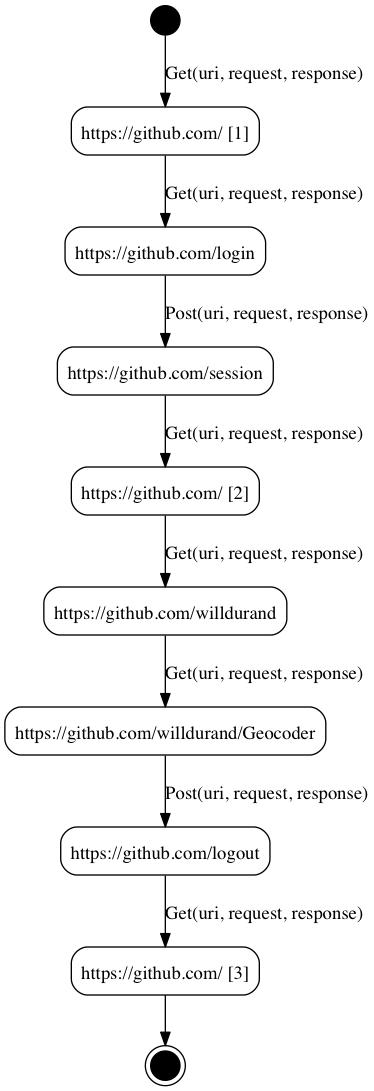
\includegraphics[width=0.8\linewidth]{figures/gh-iosts-1.png}

    \caption{IOSTS $\EuScript{S}_1$ obtained after the
    application of Layer 2.}
    \label{fig:github:iosts:1}
\end{minipage}
\begin{minipage}{.5\textwidth}
    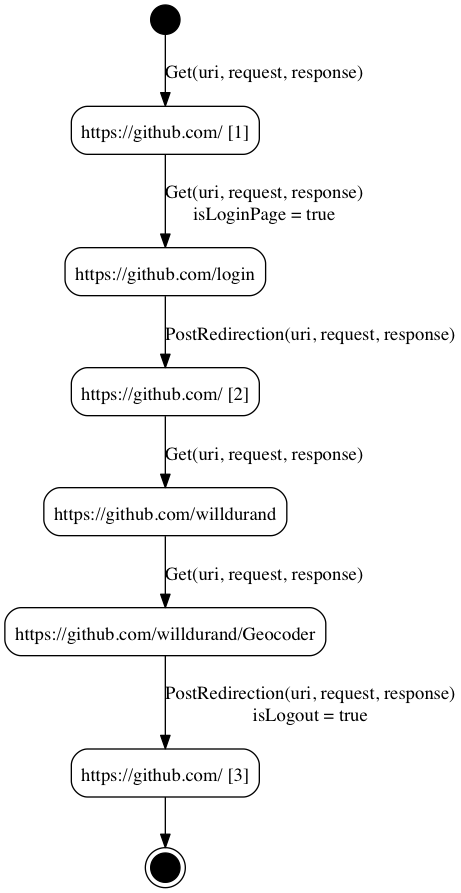
\includegraphics[width=1.0\linewidth]{figures/gh-iosts-2.png}

    \caption{IOSTS $\EuScript{S}_2$ obtained after the
    application of Layer 3.}
    \label{fig:github:iosts:2}
\end{minipage}
\end{figure}

\subsection{Layers 3-N: IOSTS abstraction}
\label{sec:modelinf:webapps:L4}

As stated earlier, the rules of the upper layers analyze the
transitions of the current IOSTS for trying to enrich its
semantics while reducing its size. Given an IOSTS
$\EuScript{S}_1$, every next layer carries out the following
steps:

\begin{enumerate}
\item Apply the rules of the layer and infer a new knowledge base
(new IOSTS $\EuScript{S}_i$, $i\geq 2$);

\item Apply a bisimulation minimization;

\item Store the resulting IOSTS.
\end{enumerate}

Without loss of generality, we now restrict the rule structure to
keep a link between the generated IOSTSs. Thereby, every rule of
Layer $i$ ($i \geq 3$) either enriches the sense of the actions
(transition per transition) or aggregates transition sequences
into one unique new transition to make the resulting IOSTS more
abstract. It results in an IOSTS $\EuScript{S}_i$ exclusively
composed of some locations of the first IOSTS $\EuScript{S}_1$.
Consequently, for a transition or path of $\EuScript{S}_i$, we
can still retrieve the concrete path of $\EuScript{S}_1$. This is
captured by the following proposition:

\begin{proposition}
\label{prop:loc:inclu}
Let $\EuScript{S}_1$ be the first IOSTS generated from the
structured trace set $ST$. The IOSTS $\EuScript{S}_i (i>1)$
produced by Layer $i$ has a location set $L_{\EuScript{S}_i}$
such that $L_{\EuScript{S}_i} \subseteq L_{\EuScript{S}_1}$.
\end{proposition}

\paragraph{Completeness, soundness, complexity.}

The knowledge base is exclusively constituted by (positive)
transition facts that have a Horn form. The rules of these layers
are Modus Ponens (soundness hypothesis). Therefore, these
inference rules are sound and complete. With regards to the (no
implicit knowledge elimination) hypothesis and to Proposition
\ref{prop:loc:inclu}, the transitions of $\EuScript{S}_i$ are
either unchanged, enriched or combined together into a new
transition. The application of these layers ends in a finite time
(finite complexity hypothesis).

\subsubsection{Layer 3}

This layers includes a (potentially empty) set of generic rules
that can be applied to a large set of applications sharing
similarities, \emph{e.g.}, applications written with the same framework
or same programming language.  This layer has two roles:

\begin{itemize}
\item The \textbf{enrichment of the meaning captured in
    transitions}. In this step, we chose to mark the transitions
    with new internal variables. These shall help deduce more
    abstract actions in the upper layers. These rules are of the
    form:

\begin{BVerbatim}
rule "Layer 3 rule"
when
  $t: Transition(conditions on action, Guard, Assign)
then
  modify ($t) {
    Assign.add(new assignment over internal variables)
  }
end
\end{BVerbatim}

$\$t$ is a transition object, like the valued actions in the
previous rules. The $modify$ keyword allows to change information
on a given object.

For example, the rules depicted in Figure \ref{fig:rule:login}
aims at recognizing the receipt of a login or logout page. The
first rule means that if the response content, which is received
after a request sent with the $GET$ method, contains a login
form, then this transition is marked as a "login page" with the
assignment on the variable $isLoginPage$;

\item The \textbf{generic aggregation of some successive
    transitions}. Here, some transitions (two or more) are
    analyzed in the conditional part of the rule. When the rule
    condition is met, then the successive transitions are replaced
    by one transition carrying a new action. These rules have the
    following form:

\begin{verbatim}
rule "Simple aggregation"
when
  $t1: Transition(
    conditions on action, Guard, ..., $lfinal := Lfinal
  )
  $t2: Transition(Linit == $lfinal, conditions)
then
  insert(new Transition(
    new Action(),
    Guard($t1.Guard, t2.Guard),
    Assign($t1.Assign, $t2.Assign),
    Linit := $t1.Linit,
    Lfinal := $t2.Lfinal
  ))
  retract($t1)
  retract($t2)
end
\end{verbatim}

Both $\$t1$ and $\$t2$ are transition objects. Transitions own
guards ($Guard$ attribute), assignments ($Assign$ attribute), but
also two locations: $Linit$ and $Lfinal$. In order to aggregate
two consecutive transitions, we have to add a condition on the
initial location of the second transition ($Linit == \$lfinal$),
\emph{i.e.} the final location of the first transition must be the
initial location of the second transition, otherwise these two
transitions are not consecutive. The $insert$ keyword in the
$then$ part is used to add a new fact to the knowledge base.
Here, we add a new transition with a more meaningful action (that
reflects the aggregation), the unions of the guards and
assignments of both transitions $\$t1$ and $\$t2$, and we set the
initial location of this new transition to the initial location
of the first transition and we set the final location of this new
transition to the final location of the section transition.

The rule given in Figure \ref{fig:rule:redirect} corresponds to a
simple transition aggregation. It aims at recognizing the
successive sending of information with a POST request followed by
a redirection to another web page.  If a request sent with the
$POST$ method has a response identified as a redirection,
(identified by the status code 301 or 302), and  a $GET$ request
comes after, both transitions are reduced into a single one
carrying the new action $PostRedirection$. Just like valued
actions, guards can be accessed: $Guard.something$ where
$something$ is a guard. The Drools Domain-Specific Language (DSL)
also provides keywords such as $contains$ or $match$ to deal with
the values.
\end{itemize}

\begin{figure}[h]
\begin{framed}
\begin{BVerbatim}
rule "Identify Login page"
when
  $t: Transition(
    Action == "GET",
    Guard.response.content contains('login-form')
  )
then
  modify ($t) {
    Assign.add("isLoginPage := true")
  }
end
\end{BVerbatim}
\end{framed}

\begin{framed}
\begin{BVerbatim}
rule "Identify Logout action"
when
  $t: Transition(
    Action == "GET",
    Guard.uri matches("/logout")
  )
then
  modify ($t1) {
    Assign.add("isLogout := true")
  }
end
\end{BVerbatim}
\end{framed}

    \caption{Login page and logout action recognition rules. The
    first rule adds a new assignment to any transition having a
    response's content containing a login form. The second
    transition adds a new assignment to all transitions where
    the $uri$ (guard) matches $/logout$, identifying logout
    actions.}
    \label{fig:rule:login}
\end{figure}

\begin{figure}[h]
\begin{framed}
\begin{BVerbatim}
rule "Identify Redirection after a POST"
when
  $t1: Transition(
    Action == "POST",
    (Guard.response.status = 301 or Guard.response.status = 302),
    $l1final := Lfinal
  )
  $t2: Transition(
    Action == "GET", Linit == $l1final
  )
then
  insert(new Transition(
    "PostRedirection",
    Guard($t1.Guard, $t2.Guard),
    Assign($t1.Assign, $t2.Assign),
    $t1.Linit,
    $t2.Lfinal
  )
  retract($t1)
  retract($t2)
end
\end{BVerbatim}
\end{framed}

\caption{An inference rule that represents a simple aggregation
identifying a redirection after a $POST$ request, leading to the
creation of a new $PostRedirection$ transition.}
\label{fig:rule:redirect}
\end{figure}

\begin{example}
When we apply these rules on the IOSTS example given in Figure
\ref{fig:github:iosts:1}, we obtain a new IOSTS illustrated in
Figure \ref{fig:github:iosts:2}. Its size is reduced since it has
6 transitions instead of 8 previously. Nonetheless, this new
IOSTS does not precisely reflect the initial scenario yet. Rules
deducing more abstract actions are required. These are found in
the next layer.
\end{example}

\subsubsection{Layer 4}

This layer aims at inferring a more abstract model composed of
more expressive actions and whose size should be reduced. Its
rules may have different forms:

\begin{itemize}
\item They can be applied to a single transition only. In this
case, the rule replaces the transition action to add more sense
to the action. The rule given in Figure \ref{fig:rule:deauth} is
an example, which recognizes a user de-authentication, and adds a
new action $Deauthentication$. This rule means that if a
$PostRedirection$ action is triggered against a "Logout" endpoint
(given by the variable \textit{isLogout} added by Layer 3), then
this is a "de authentication";

\item The rules can also aggregate several successive transitions
up to complete paths into one transition labeled by a more
abstract action. For instance, the rule illustrated in Figure
\ref{fig:rule:auth} recognizes a user authentication thanks to
the variable $isLoginPage$ added by Layer 3. This rule means that
if a "login" page is displayed, followed by a redirection
triggered by a $POST$ request, then this is an authentication
step, and the two transitions are reduced into a single one
composed of the action $Authentication$.
\end{itemize}

\begin{figure}[h]
\begin{framed}
\begin{BVerbatim}
rule "Identify Deauthentication"
when
  $t: Transition(
    action == "PostRedirection",
    Assign contains "isLogout := true"
  )
then
  modify ($t) {
    $t.setAction("Deauthentication")
  }
end
\end{BVerbatim}
\end{framed}

    \caption{This rule recognizes an action that we call
    "deauthentication", \emph{i.e.} when a user logs out.}
    \label{fig:rule:deauth}
\end{figure}

\begin{figure}[h]
\begin{framed}
\begin{BVerbatim}
rule "Identify Authentication"
when
  $t1: Transition(
    Action == "GET",
    Assign contains "isLoginPage := true",
    $t1final := Lfinal
  )
  $t2: Transition(
    Action == "PostRedirection",
    Linit == $t1final
  )
then
  insert(new Transition(
    "Authentication",
    Guard($t1.Guard,$t2.Guard),
    Assign($t1.Assign, $t2.Assign),
    $t1.Linit,
    $t2.Lfinal
  )
  retract($t1)
  retract($t2)
end
\end{BVerbatim}
\end{framed}

    \caption{Authentication recognition by leveraging information
    carried by the rule given in Figure \ref{fig:rule:redirect}.
    When a user browses a web page containing a login form,
    following by a $PostRedirection$, this is an $Authentication$
    action.}
    \label{fig:rule:auth}
\end{figure}

Other rules can also be application-specific, so that these bring
specific new knowledge to the model. For instance, the GitHub web
application has a dedicated URL grammar (a.k.a. routing system).
GitHub users own a profile page that is available at:
\textit{https://github.com/\{username\}} where \textit{\{username\}}
is the nickname of the user. However, some items are reserved,
\emph{e.g.}, \textit{edu} and \textit{explore}. The rule given in Figure
\ref{fig:rule:gh-profile} is based upon this structure and
produces a new action $ShowProfile$ offering more sense.
Similarly, a GitHub page describing a project has a URL that
always matches the pattern:
\textit{https://github.com/\{username\}/\{project\_name\}}. The
rule given in Figure \ref{fig:rule:gh-project} captures this
pattern and derives a new action named $ShowProject$.

\begin{figure}
\begin{framed}
\begin{BVerbatim}
rule "GitHub profile pages"
when
  $t: Transition(
    action == "GET",
    (Guard.uri matches "/[a-zA-Z0-9]+$",
     Guard.uri not in [ "/edu", "/explore" ])
  )
then
  modify ($t) { $t.setAction("ShowProfile") }
end
\end{BVerbatim}
\end{framed}

    \caption{User profile recognition. This rule is specific to the
    application under analysis, and works because profile pages are
    anything but \textit{/edu} and \textit{/explore}.}
    \label{fig:rule:gh-profile}
\end{figure}

\begin{figure}
\begin{framed}
\begin{BVerbatim}
rule "GitHub project pages"
when
  $t: Transition(
    action == "GET",
    Guard.uri matches "/[a-zA-Z0-9]+/.+$",
    $uri := Guard.uri
  )
then
  String s = ParseProjectName($uri)
  modify ($t) {
    $t.setAction("ShowProject")
    Assign.add("ProjectName := " + s)
  }
end
\end{BVerbatim}
\end{framed}

\caption{Project choice recognition. Here again, this is a
specific rule for the application under analysis that works
because the routing of this application defines projects at URIs
matching \textit{/\{username\}/\{project name\}}.}
\label{fig:rule:gh-project}
\end{figure}

\begin{example}
The application of the four previous rules leads to the final
IOSTS depicted in Figure \ref{fig:github:iosts:4}. Now, it can be
used for application comprehension since most of its actions have
a precise meaning and clearly describe the application's
behaviors.
\end{example}

\begin{figure}[ht]
    \begin{center}
    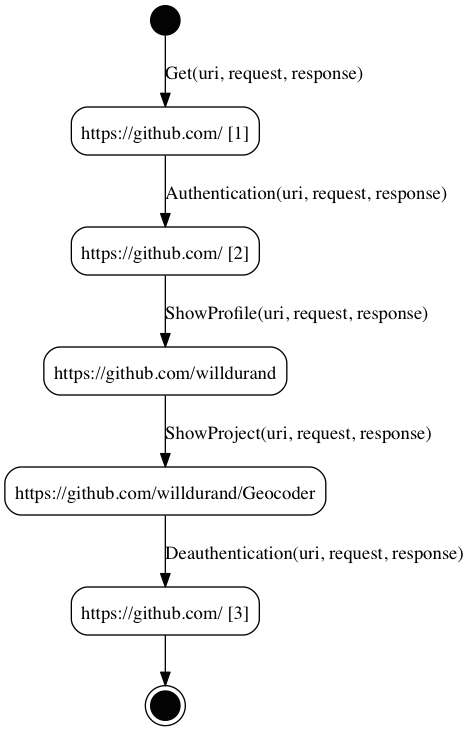
\includegraphics[width=0.6\linewidth]{figures/gh-iosts-41.png}
    \caption{The final IOSTS $\EuScript{S}_3$ obtained after the
    application of Layer 4.}
    \label{fig:github:iosts:4}
    \end{center}
\end{figure}

%%%%%%%%%%%%%%%%%%%%%%%%%%%%%%%%%%%%%%%%%%%%%%%%%%%%%%%%%%%%%%%%

\section{Getting more complete models with strategies}
\label{sec:modelinf:webapps:strategy}

Since the inference of our models depends on both the amount and
the quality of the collected traces, these models are said
partial. In order to improve the completeness of our inferred
models, we rely on an automatic testing technique (that is,
crawling) to interact with the application. This is the role of
the Robot explorer, driven by the Models generator.

Rather than using a static traversal strategy as in
\cite{Memon:2003,concolicandroid12,crawljax:tweb12,
Amalfitano:2012:UGR:2351676.2351717, WPX13}, we propose the
addition of an orthogonal layer in the Models generator to
describe any kind of exploration strategy by means of rules.

The simplified Algorithm of the Strategy layer is given in
Algorithm \ref{exploration-strategy}. The latter applies the
rules on any stored IOSTS $\EuScript{S}_i$. It emerges a
location list $Loc$ that are marked with "explored" by the rules
to avoid re-using them twice (line 4). Then, the algorithm goes
back to the first generated IOSTS $\EuScript{S}_1$ in order to
extract one complete and executable path $p$ ended by a location
$l$ of $Loc$ (line 5). This step is sound since all the locations
of $\EuScript{S}_i$ belong to the location set of
$\EuScript{S}_1$ (Proposition \ref{prop:loc:inclu}). Such an
IOSTS preamble is required by the Robot explorer for trying to
reach the location $l$ by executing every action of $p$. The
algorithm finally returns a list of paths $List$, which is sent
to the Robot explorer. The exploration ends once all the
locations of $\EuScript{S}_i$ or of $\EuScript{S}_1$ are visited
(line 3). The algorithm only returns unexplored locations even
if, while the execution of the algorithm, the IOSTS
$\EuScript{S}_i$ has been regenerated several times since the
marked locations are also stored in the set $L$. Hence, if a
location of $\EuScript{S}_i$ is chosen a second time by the
rules, the algorithm checks if it has been previously visited
(line 7).

\begin{algorithm}
\SetKwInOut{Input}{input} \SetKwInOut{Output}{output}

\Input{IOSTS $\EuScript{S}_1$, $\EuScript{S}_i$}
\Output{List of preambles}

$L:=\emptyset$ List of explored locations of $\EuScript{S}_1$\;
BEGIN\;
\While{$L \neq L_{\EuScript{S}_1}$ and $L \neq L_{\EuScript{S}_i}$ }
{
Apply the rules on $\EuScript{S}_i$ and extract a  Location List $Loc$\;
Go back to $\EuScript{S}_1$\;

\ForEach{$l \in Loc$}{
\If{$l \notin L$}
{Compute a preamble $p$ from $l0_{\EuScript{S}_1}$ which reaches $l$\;

$L:= L \cup \{l\}$\;
$List:= List \cup  \{p\}$\;
}
%\Else{Repeat 1)}
}
}
END\;

\caption{Exploration strategy}
\label{exploration-strategy}
\end{algorithm}

The rules of the Strategy layer can encode different strategies.
We propose two examples below:

\begin{itemize}
    \item \textbf{Classical traversal strategies} (Depth-first
        search, Breadth-first search) can still be established.
        For example, Figure \ref{fig:rule:bfs} depicts two rules
        expressing the choice the next location to explore in a
        breadth-wise order first. First, the initial location
        $l0$ is chosen and marked as explored (rule BFS).  Then,
        the transitions having an initial location marked as
        explored and a final location not yet explored are
        collected by the rule BFS2, except for the transitions
        carrying an HTTP error (response status upper or equal to
        400).  The $accumulate$ keyword is a Drools function that
        allows to operate on sets of data, which we used to
        transcribe the previous sentence.  The selected locations
        are marked as explored in the IOSTS $\EuScript{S}_i$ with
        the method $SetExplored$ in the "then" part of the rule;

    \item \textbf{Semantic-driven strategies} could also be
        applied, when the meaning of some actions is
        recognizable. For instance, for e-commerce applications,
        the login step and the term "buy" are usually important.
        Thereby, a strategy targeting firstly the locations of
        transitions carrying theses actions can be defined by the
        rule "semantic-driven strategy" given in Figure
        \ref{fig:rule:semdriven}.  It is manifest that the
        semantic-driven strategy domain can be tremendously vast
        since it depends on the number of recognized actions and
        on their relevance.
\end{itemize}

\begin{figure}[h]
\begin{framed}
\begin{BVerbatim}
rule "BFS"
when
  $l: Location(name == l0, explored == false)
then
  $l.SetExplored()
end
\end{BVerbatim}
\end{framed}

\begin{framed}
\begin{BVerbatim}
rule "BFS2"
when
  $Loc: ArrayList<Location>() from accumulate(
    $t: Transition(Guard.response.status > 199
      && Guard.response.status < 400
      && Linit.explored == true
      && Lfinal.explore==false
    ),
    init(ArrayList<Transition> Loc = new ArrayList<Transition>()),
    action(Loc.add($t.Lfinal)),
    result(Loc)
  )
then
  Loc.SetExplored()
end
\end{BVerbatim}
\end{framed}

\caption{Two rules used to implement a Breadth-first search (BFS)
exploration strategy.}
\label{fig:rule:bfs}
\end{figure}

\begin{figure}[h]
\begin{framed}
\begin{BVerbatim}
rule "semantic-driven strategy"
when
  $t: Transition (
    Assign contains "isLogin := true"
    or Guard.response matches "*buy*"
  )
then
  ArrayList Loc = new ArrayList()
  Loc.add($t.Linit, $t.Lfinal)
  Loc.SetExplored()
end
\end{BVerbatim}
\end{framed}

\caption{A semantic-driven exploration strategy that focuses on
the term "buy" in the HTTP responses, \emph{i.e.} displayed the web
pages.}
\label{fig:rule:semdriven}
\end{figure}

Many other strategies could be defined in relation to the desired
result in terms of model generation and application coverage.
Other criteria, \emph{e.g.}, the number of UI elements per Graphical User
Interface (GUI) or the number of observed crashes could also be
taken into consideration.

%%%%%%%%%%%%%%%%%%%%%%%%%%%%%%%%%%%%%%%%%%%%%%%%%%%%%%%%%%%%%%%%%

\section{Implementation and experimentation}
\label{sec:modelinf:webapps:exp}

We implemented this technique in a prototype tool called
\textit{Autofunk}. A user interacts with \textit{Autofunk} through a web
interface and either gives a URL  or a file containing traces.
These have to be stored in the HTTP Archive (HAR) format as it is
the defacto standard to describe HTTP traces, used by various
HTTP related tools. Such traces can be obtained from many HTTP
monitoring tools (Mozilla Firefox or Google Chrome included).
Then, \textit{Autofunk} produces IOSTS models, which are stored in a
database. The last model is depicted in the web interface.

The JBoss Drools Expert tool has been chosen to implement the
rule-based system. Such an engine leverages Object-Oriented
Programming in the rule statements and takes knowledge bases
given as Java objects (Location, Transition, GET, POST objects in
this work).

The GitHub website \footnote{\url{https://github.com/}} is an example
of application giving significant results. We recorded a trace
set composed of 840 HTTP requests / responses. Then, we applied
\textit{Autofunk} to them with a Models generator composed of 5 layers
gathering 18 rules whose 3 are specialized to GitHub. After
having performed trace filtering (Layer 1), we obtained a first
IOSTS tree composed of 28 transitions. The next 4 layers
automatically inferred a last IOSTS tree $\EuScript{S}_4$, given
in Figure \ref{fig:git:iosts}, that is composed of 12 transitions
from which 9 have a clear and intelligible meaning. Layers 4 and
5 include inference rules that are specific to GitHub. For other
websites, these rules cannot be reused and have to be rewritten.

\begin{figure}[ht]
    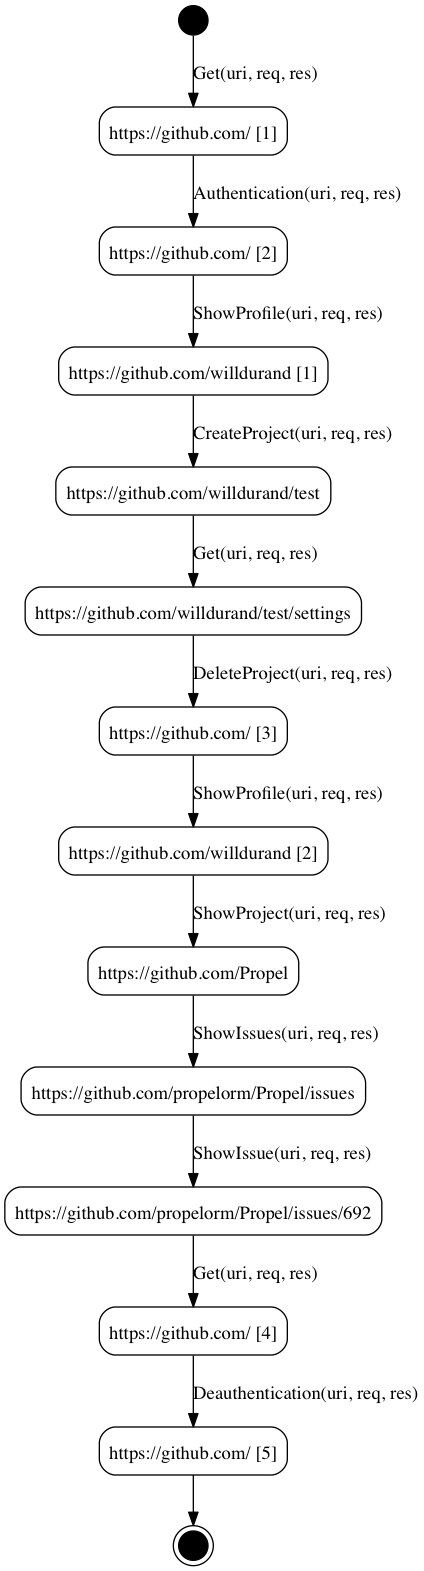
\includegraphics[width=.45\textwidth]{figures/gh-2-4-bis.png}

    \caption {This model is the IOSTS $\EuScript{S}_4$ obtained
    from a trace set composed of 840 HTTP requests and responses,
    and after the application of 5 layers gathering 18 rules.}
    \label{fig:git:iosts}
\end{figure}

%%%%%%%%%%%%%%%%%%%%%%%%%%%%%%%%%%%%%%%%%%%%%%%%%%%%%%%%%%%%%%%%%

\section{Conclusion}
\label{sec:modelinf:webapps:conclusion}

In this chapter, we presented an original approach combining
model inference, expert systems, and automatic testing to derive
IOSTSs models by means of a model transformation using inference
rules.  We chose a minimization technique over existing
algorithms such as gkTail and KLFA to keep exactness of the
inferred models. Our proposal yields several models, reflecting
different levels of abstraction of the same application with the
use of inference rules that capture the knowledge of an expert.
The first contribution lies in the flexibility and scalability
brought by the inference rules since they can be applied to
several applications or on a single application only when the
rules are specific. The whole framework has not to be
re-implemented for each application, but inference rules have to.
Our approach can be applied to event-driven applications since
our framework supports their exploration. Furthermore, it can
also be applied to other kinds of application as far as they
produce traces.

Combining expert systems (gathering knowledge) and formal models
is really interesting but this is not a silver bullet. Indeed,
writing rules is still an heavy task, and thus not suitable as
is. It can be as difficult as writing a formal model, hence the
need for an automated way to write the rules of Layers 3 to N.
Ideally, the framework itself should generate a set of rules,
\emph{e.g.}, using a machine learning technique.

The first results on model inference were very encouraging, so we
decided to rework our architecture to build a better framework on
top of this one in order to construct models of production
systems. That is the purpose of the next chapter.
